\newpage

\section*{ $^{47}$Ti(n,p)$^{47}$Sc }

Power Level: 100 kW(th) \\
Time at Power: 60.0 m \\
Wait Time: 60.0 m \\
Counting Time: 30.0 m \\
Total Activity at Removal: 7.53e-02 $\mu Ci$

\begin{table*}[h]
\centering
\begin{tabular}{ |c|c|c|c|c|c| }
 \hline
 Position & Mass $mg$ & Counting Activity $\mu Ci$ & Area (Counts) & Error \% \\
 \hline 
 1 & 5.50 & 1.72e-02 & 8.20e+04 & 0.3493 \\ 
\hline
 2 & 5.10 & 2.49e-02 & 1.19e+05 & 0.2902 \\ 
\hline
 3 & 5.10 & 2.28e-02 & 1.09e+05 & 0.3031 \\ 
\hline
 4 & 5.30 & 1.01e-02 & 4.81e+04 & 0.4560 \\ 
\hline
\end{tabular}
\end{table*}

\begin{figure}[h]
\centering
\begin{subfigure}{.5\textwidth}
  \centering
     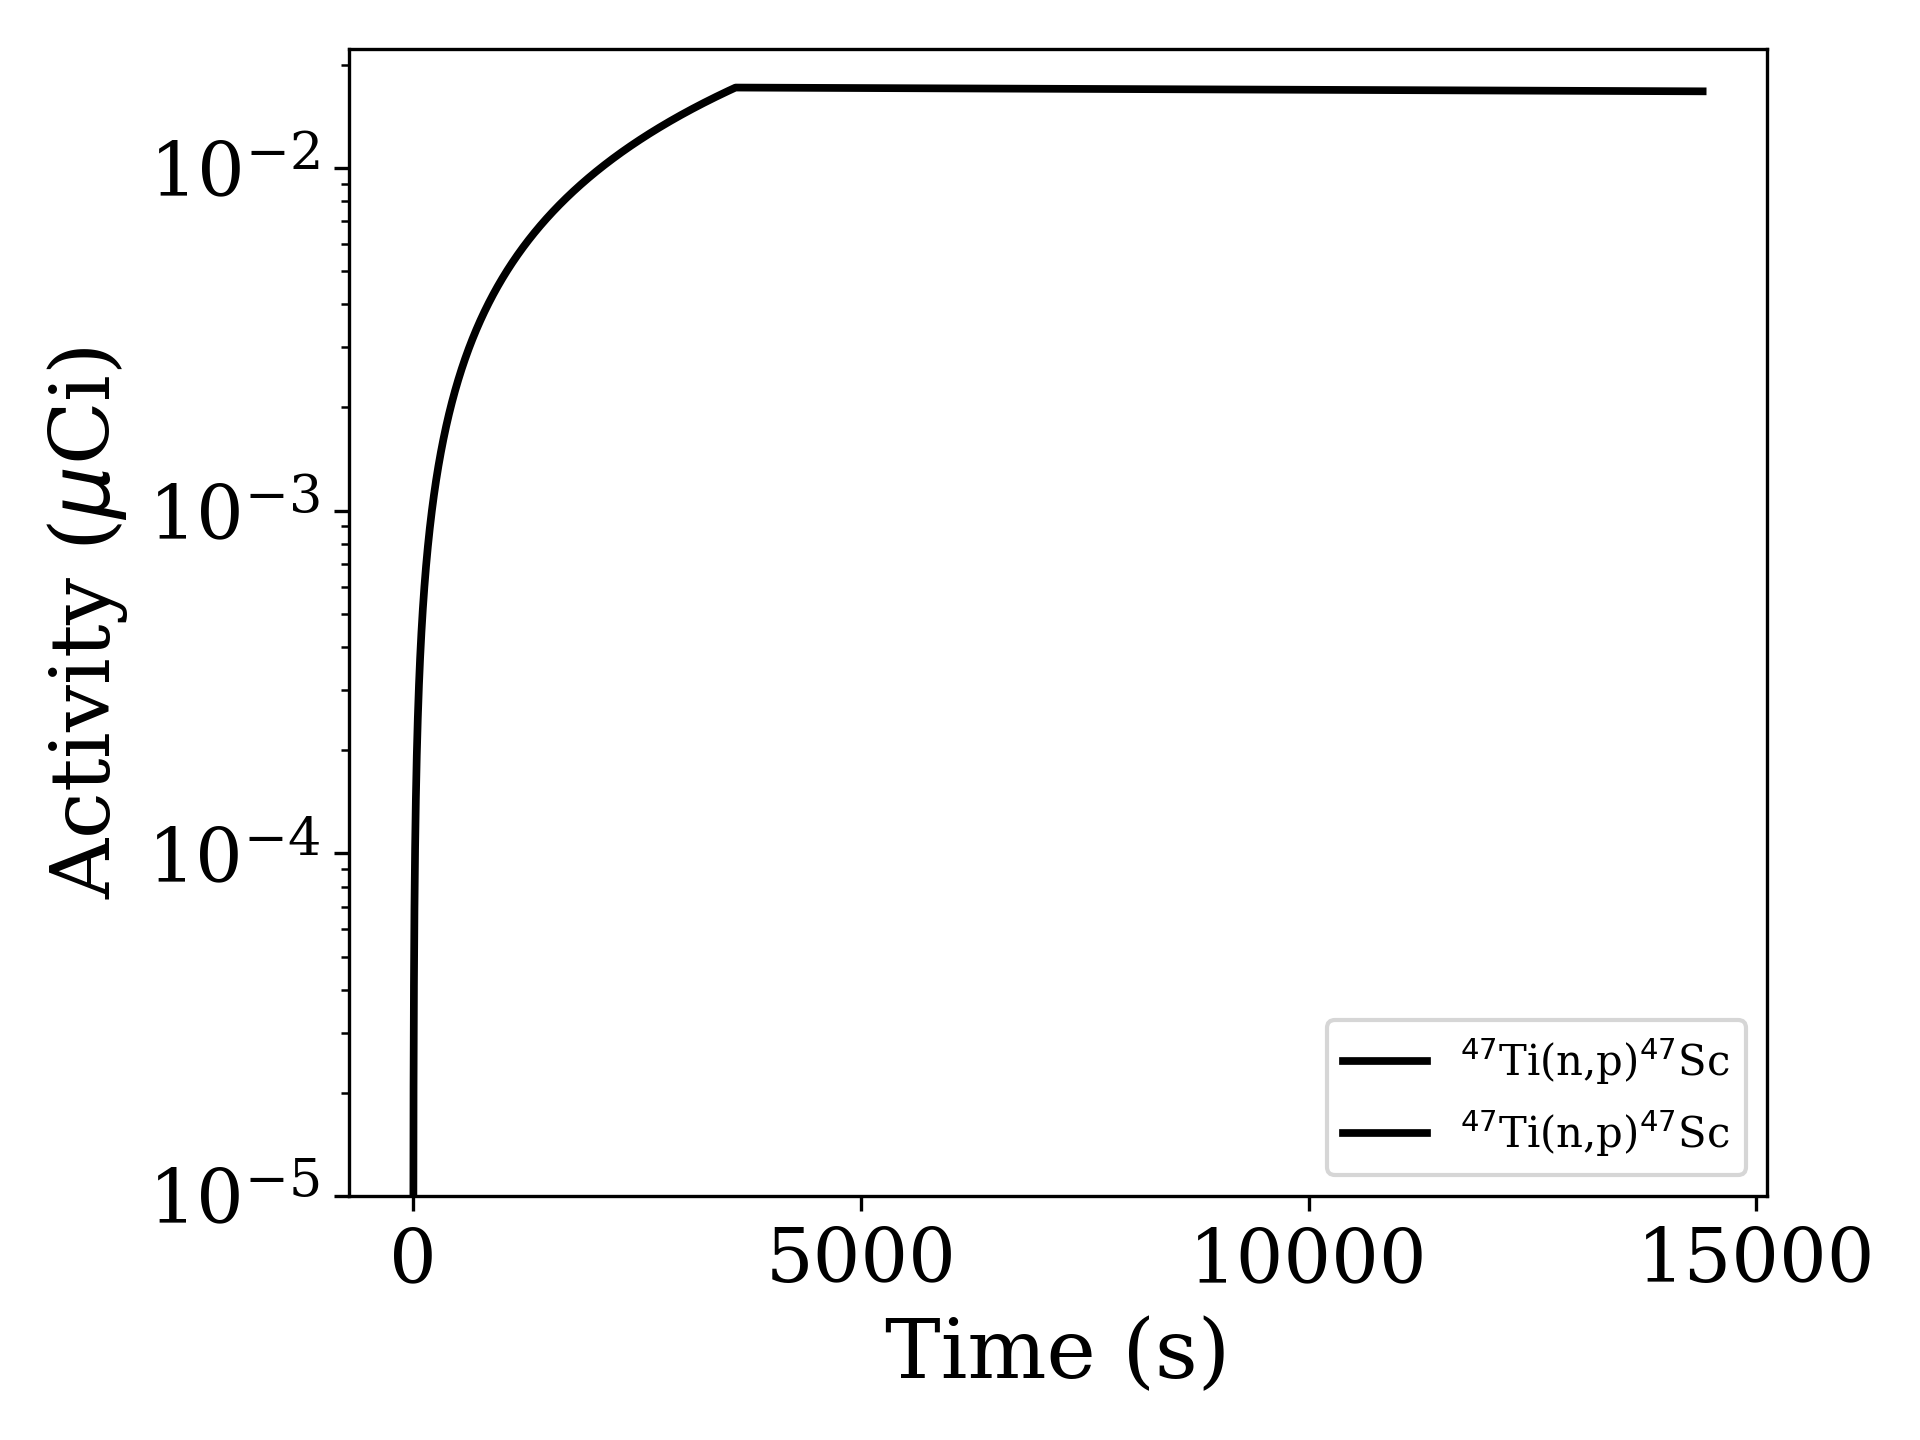
\includegraphics[width=.8\textwidth]{plot/Ti-47(n,p)Sc-47_wisconsin1} 

  \caption{Activity}
\end{subfigure}%
\begin{subfigure}{.5\textwidth}
  \centering
     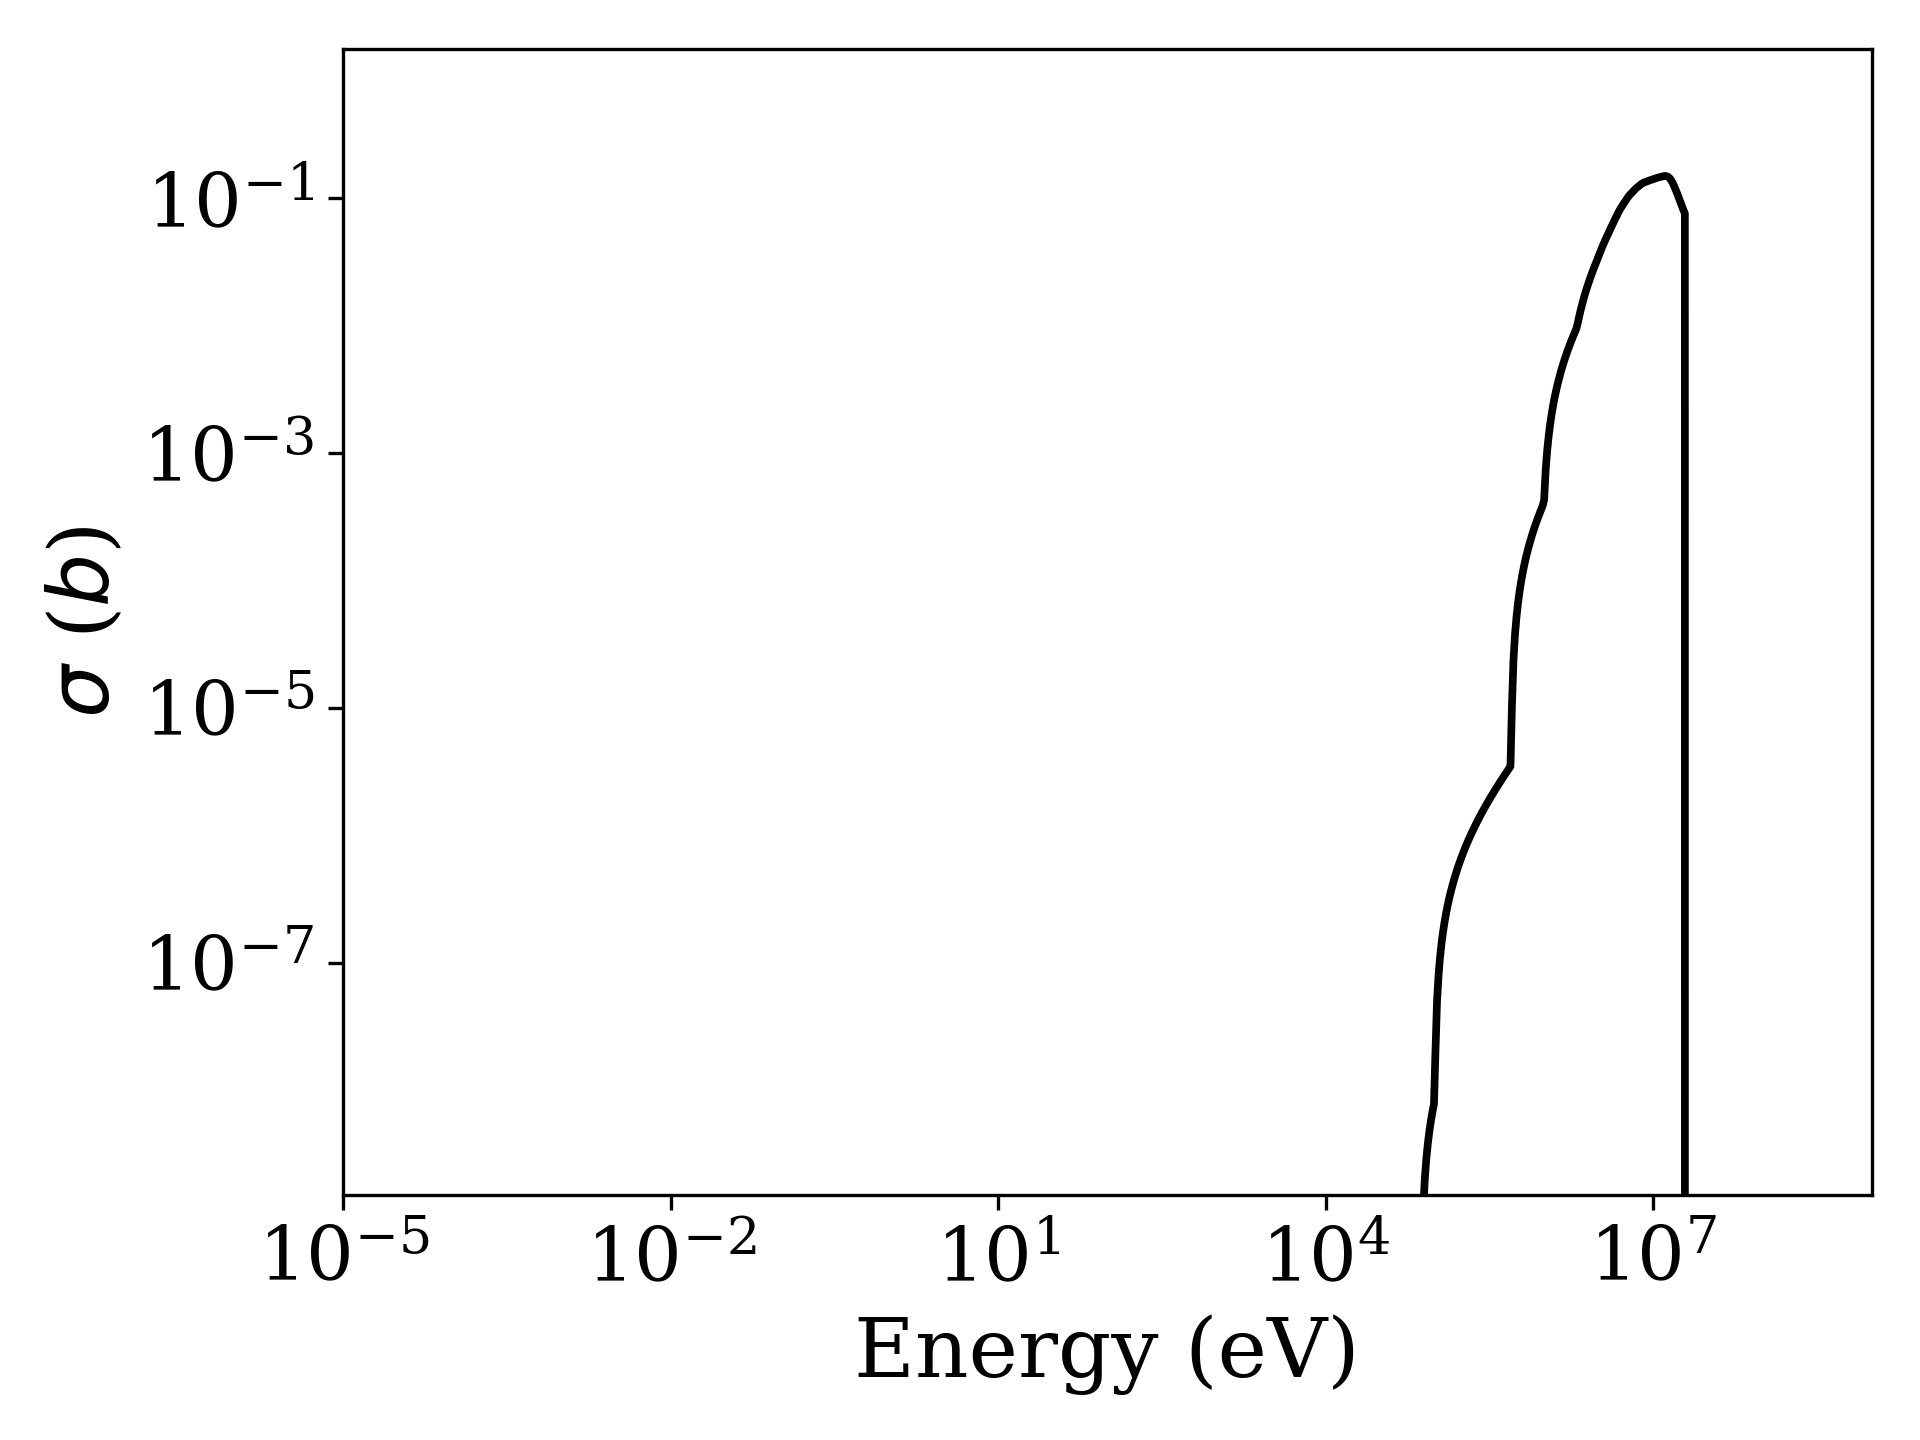
\includegraphics[width=.8\textwidth]{plot/Ti-47(n,p)Sc-47} 

  \caption{Cross Section}
\end{subfigure}
\end{figure}

\begin{table*}[h]
\centering
\begin{tabular}{ |c|c|c|c|c|c|c| }
 \hline
 Reaction & T$_{1/2}$ & ROI (eV) & Important Gammas (keV) \\
 \hline 
 $^{47}$Ti(n,p)$^{47}$Sc &  3.4 d & 1.68e+06, 8.17e+06 & 160(0.73) \\ 
\hline
\end{tabular}
\end{table*}
